
\begin{figure}
  \begin{center}
    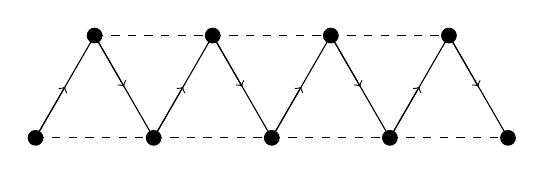
\begin{tikzpicture}
      \fill (0,0) circle[radius = 0.1];
      \fill (1.5,0) circle[radius = 0.1];
      \fill (3,0) circle[radius = 0.1];
      \fill (4.5,0) circle[radius = 0.1];
      \fill (6,0) circle[radius = 0.1];

      \draw[dashed] (0,0)--(1.5,0);
      \draw[dashed] (1.5,0)--(3,0);
      \draw[dashed] (3,0)--(4.5,0);
      \draw[dashed] (4.5,0)--(6,0);
      \draw[->] (0,0)--(60:0.75);
      \draw[->] (1.5,0)--++(60:0.75);
      \draw[->] (3,0)--++(60:0.75);
      \draw[->] (4.5,0)--++(60:0.75);
      \draw (0,0)--(60:1.5);
      \draw (1.5,0)--++(60:1.5);
      \draw (3,0)--++(60:1.5);
      \draw (4.5,0)--++(60:1.5);
      
      \begin{scope}[shift=(60:1.5)]
        \fill (0,0) circle[radius = 0.1];
        \fill (1.5,0) circle[radius = 0.1];
        \fill (3,0) circle[radius = 0.1];
        \fill (4.5,0) circle[radius = 0.1];
        \draw[dashed] (0,0)--(1.5,0);
        \draw[dashed] (1.5,0)--(3,0);
        \draw[dashed] (3,0)--(4.5,0);
        \draw[->] (0,0)--(-60:0.75);
        \draw[->] (1.5,0)--++(-60:0.75);
        \draw[->] (3,0)--++(-60:0.75);
        \draw[->] (4.5,0)--++(-60:0.75);
        
        \draw (0,0)--(-60:1.5);
        \draw (1.5,0)--++(-60:1.5);
        \draw (3,0)--++(-60:1.5);
        \draw (4.5,0)--++(-60:1.5);
      \end{scope}
      
    \end{tikzpicture}
    \caption{zig-zag conformation}
    \label{TTT_zigzag}
  \end{center}
\end{figure}


In this section, we consider Problem~\ref{prob:det_unary_length} at delay 1. Our result, cases of arity 1 and 3 can only yield finite structures of size $O (n)$, and cases of arity 4 and more can only yield finite structures which is size of $O (n^2)$, and a case of arity 2 can yield infinite structures but they are only the zig-zag conformation shown in Fig.~\ref{TTT_zigzag}. 

%In this section, we prove that unary oritatami system can form infinitely at delay 1 and arity 2 deterministically and moreover that the only infinite conformations which its oritatami system can yield is only the zig-zag conformation shown in Fig.\ref{TTT_zigzag}. 


Let $\Xi = (\Sigma, R, \delta, \alpha, \sigma, w)$ be a deterministic oritatami system of delay 1. 
For $i \geq 0$ let $C_i$ be the unique elongation of $\sigma$ by $w[1..i]$, that is, foldable by $\Xi$. Hence $C_0 = \sigma$.

\begin{figure}
  \begin{center}
    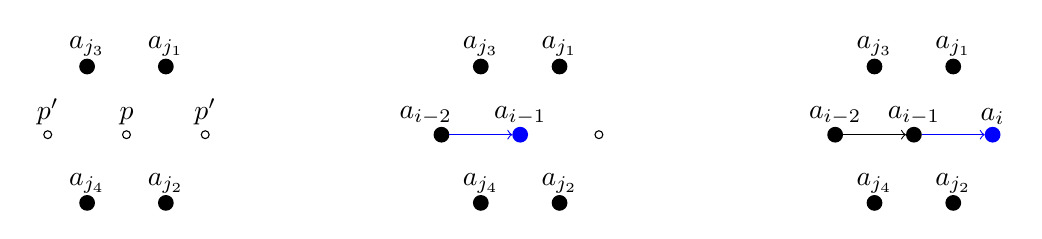
\begin{tikzpicture}
      \draw (0:0) circle [radius=0.05];
      \draw (0:1) circle [radius=0.05];
      \draw (180:1) circle [radius=0.05];
      \node[above] at (0:1) { $p^\prime$ };
      \node[above] at (0:0) { $p$ };
      \node[above] at (180:1) { $p^\prime$ };
      
      \fill (60 : 1) circle [radius=0.1];
      \fill (-60 : 1) circle [radius=0.1];
      \fill (120 : 1) circle [radius=0.1];
      \fill (-120 : 1) circle [radius=0.1];
      \node[above] at (60 :1) { $a_{j_1}$ };
      \node[above] at (-60 :1) { $a_{j_2}$ };
      \node[above] at (120 :1) { $a_{j_3}$ };
      \node[above] at (-120 :1) { $a_{j_4}$ };
      
      \begin{scope}[shift=(0:5)]
        \fill[blue] (0:0) circle [radius=0.1];
        \draw (0:1) circle [radius=0.05];
        \fill (180:1) circle [radius=0.1];
        \node[above] at (180:1.2) { $a_{i-2}$ };
        \node[above] at (0:0) { $a_{i-1}$ };
        \draw[->, blue] (180:0.9) -- (180:0.1);
        
        \fill (60 : 1) circle [radius=0.1];
        \fill (-60 : 1) circle [radius=0.1];
        \fill (120 : 1) circle [radius=0.1];
        \fill (-120 : 1) circle [radius=0.1];
        \node[above] at (60 :1) { $a_{j_1}$ };
        \node[above] at (-60 :1) { $a_{j_2}$ };
        \node[above] at (120 :1) { $a_{j_3}$ };
        \node[above] at (-120 :1) { $a_{j_4}$ };
      \end{scope}
      \begin{scope}[shift=(0:10)]
        \fill (0:0) circle [radius=0.1];
        \fill[blue] (0:1) circle [radius=0.1];
        \fill (180:1) circle [radius=0.1];
        \node[above] at (180:1) { $a_{i-2}$ };
        \node[above] at (0:0) { $a_{i-1}$ };
        \node[above] at (0:1) { $a_i$ };
        \draw[->] (180:0.9) -- (180:0.1);
        \draw[->,blue] (0:0.1) -- (0:0.9);
        
        \fill (60 : 1) circle [radius=0.1];
        \fill (-60 : 1) circle [radius=0.1];
        \fill (120 : 1) circle [radius=0.1];
        \fill (-120 : 1) circle [radius=0.1];
        \node[above] at (60 :1) { $a_{j_1}$ };
        \node[above] at (-60 :1) { $a_{j_2}$ };
        \node[above] at (120 :1) { $a_{j_3}$ };
        \node[above] at (-120 :1) { $a_{j_4}$ };
      \end{scope}
    \end{tikzpicture} 
    \caption{Through a tunnel section}
    \label{TTT_tunnel_intro}
  \end{center}
\end{figure}

\begin{figure}
  \begin{center}
    \begin{tabular}{ccc}
      
      \begin{minipage}{0.3\hsize}
        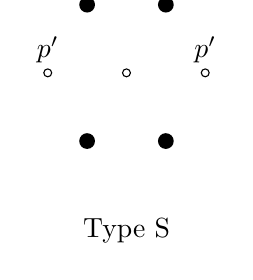
\begin{tikzpicture}
          \begin{scope}[xshift=2cm, yshift=2cm]
            \draw(0,0) circle [radius=0.05];
            \node[above] at (180:1) {$p^\prime$};
            \node[above] at (0:1) {$p^\prime$};

            \foreach \theta in {0,180}{
              \draw[transform canvas={shift=(\theta:1)}](0,0) circle [radius=0.05];
            }
            
            \foreach \theta in {60,-60,120,-120}{
              \fill[transform canvas={shift=(\theta:1)}](0,0) circle [radius=0.1];
            }
          \end{scope}

          \node at (2,0) {Type S};
        \end{tikzpicture}
      \end{minipage}

      \begin{minipage}{0.3\hsize}
        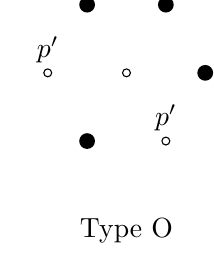
\begin{tikzpicture}

          \begin{scope}[xshift=2cm, yshift=2cm]
            \draw(0,0) circle [radius=0.05];
            \node[above] at (180:1) {$p^\prime$};
            \node[above] at (-60:1) {$p^\prime$};

            \foreach \theta in {-60,180}{
              \draw[transform canvas={shift=(\theta:1)}](0,0) circle [radius=0.05];
            }
            
            \foreach \theta in {0,60,120,-120}{
 	            \fill[transform canvas={shift=(\theta:1)}](0,0) circle [radius=0.1];
            }
          \end{scope}

          \node at (2,0) {Type O};
        \end{tikzpicture}
      \end{minipage}

      \begin{minipage}{0.3\hsize}
        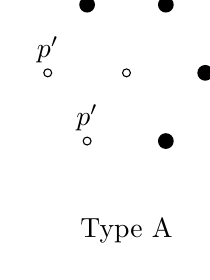
\begin{tikzpicture}

          \begin{scope}[xshift=2cm, yshift=2cm]
            \draw(0,0) circle [radius=0.05];
            \node[above] at (180:1) {$p^\prime$};
            \node[above] at (-120:1) {$p^\prime$};

            \foreach \theta in {-120,180}{
              \draw[transform canvas={shift=(\theta:1)}](0,0) circle [radius=0.05];
            }
            
            \foreach \theta in {0,60,-60,120}{
              \fill[transform canvas={shift=(\theta:1)}](0,0) circle [radius=0.1];
            }
          \end{scope}

          \node at (2,0) {Type A};
        \end{tikzpicture}
      \end{minipage}
      
    \end{tabular}
    \caption{Tunnel sections of all possible three types: straight (Type S), obtuse turn (Type O), and acute turn (Type A).}
    \label{fig:TTT_tunnel}
  \end{center}
\end{figure}

At delay 1, a bead cannot collaborate with its successors in order to stabilize itself. 
In fact, there are just two ways for a bead to get stabilized at delay 1 (or the bead has no place to be stabilized around so that the system halts). 
One is to be bound and the other is through a 1-in-1-out structure called the tunnel section. 
See Fig.~\ref{fig:TTT_tunnel}. 
A \textit{tunnel section} consists of four beads that occupy four neighbors of one free point. 
The behavior of a deterministic oritatami system at delay 1 can be described by a sequence of $S$ of $b$ (bound), $t_s$ (straight tunnel section), $t_o$ (obtuse-turn tunnel section), and $t_a$ (acute-turn tunnel section); priority is given to tunnel, that is, $S[i]$ is $t_s$ (resp.~$t_o$, $t_a$) if the $i$-th bead of the system is stabilized not only by being bonded but also through a straight (resp. obtuse-turn, acute-turn) tunnel section. 
We let $S$ take the value $\blacksquare$ for halt (due to the lack of free neighbors). 

Assume that four of the six neighbors of a point $p$ are occupied by beads $a_{j_1},a_{j_2},a_{j_3},a_{j_4}$ while the other two are free. We call such a point $p$ the $inside\ of\ a\ tunnel$ and points $p^\prime$ the $entrance\ of\ a\ tunnel$ except when $p^\prime$ is inside of a tunnel. If the beads $w[i-2]$ and $w[i-1]$ are stabilized respectively at one of the two free neighbors and at $p$ one after another, then the next bead $w[i]$ cannot help but be stabilized at the other free neighbor. In this way, $w[i]$ can get stabilized without being bound.

%If a bead is stabilized through a tunnel section, then it can provide some bonds. Let us consider bonds of $C_i$. $C_i$ is represented $C = (W,P,H)$ where $|W| = i + n$ $C_i$ contains $\alpha \cdot (i + n) - 2|H|$ bonds because $C_i$ consists of $i + n$ beads and a bead has just $\alpha$ bonds and then $2 |H|$ of the those bonds are already used. However, even if a bead has an available bond, $w[j]$ $(j > i)$ might not be able to use this bond because the bond has possibility that it is blocked by transcripts $w[i+1..j-1]$. Number of $binding\ capabilities$ does not contain that case so that it is at most $\alpha \cdot (i + n) - 2|H|$.

We say that point $p$ is reachable from a conformation $C$ if there exists a directed path $P^\prime$ from the last point of $C$ that does not cross the path of $C$. 
Taking this reachability into account, we define the \textit{binding capability} of a conformation as the number of free bonds of its beads available geometrically for elongations of $C$.
It is defined formally as follows: 

\begin{definition}[binding capability]
Let $C = (P,w,H)$ be a conformation.
Let $B_k$ be $H \cap \{ (i,j) \mid \mbox{$i=k$ or $j=k$} \}$. Moreover, let $R_k$ be a set of neighbors of the point $P[k]$ that are free and reachable from $C$.
 The binding capability of $C$, denoted by $\#bc(C)$, is defined by $\sum^{|w|}_{k=1} \min \{ |B_k|, |R_k|  \}$.
\end{definition}


